% !TeX program = xelatex
\documentclass[11pt,a4paper]{ctexart}
\usepackage{amsfonts,amsmath,amssymb,graphicx,url}
\usepackage{fullpage}
\usepackage{fontspec}
\setmonofont{Courier New}
\usepackage{enumitem}
\setlist[enumerate]{font=\bfseries}
\usepackage{listings,xcolor}
\lstset{language=C}
\lstset{breaklines}
\lstset{extendedchars=false}
\definecolor{grey}{rgb}{0.8,0.8,0.8}
\definecolor{darkgreen}{rgb}{0,0.3,0}
\definecolor{darkblue}{rgb}{0,0,0.3}
%\def\lstbasicfont{\fontfamily{pcr}\selectfont\footnotesize}
\def\ttfonts{\ttfamily\footnotesize}
\lstset{%
    numbers=left,
    numberstyle=\footnotesize,%
    showstringspaces=false,
    showspaces=false,%
    tabsize=4,%
    frame=lines,
   % frame=shadowbox,
    basicstyle={\footnotesize\ttfonts},%
    keywordstyle=\color{darkblue}\bfseries,%
    identifierstyle=,%
    commentstyle=\color{darkgreen},%\itshape,%
    stringstyle=\color{black},%
    escapeinside=``
}

\setlength{\oddsidemargin}{.1in}
\setlength{\evensidemargin}{.1in}
\setlength{\topmargin}{-0.4in}

\newcommand{\heading}[5]{
   \renewcommand{\thepage}{\arabic{page}}
   \noindent
   \begin{center}
   \framebox{
      \vbox{
    \hbox to 6.2in { {\bf B62002Y-01 数据结构}
     	 \hfill #2 }
       \vspace{4mm}
       \hbox to 6.2in { {\Large \hfill #5  \hfill} }
       \vspace{2mm}
       \hbox to 6.2in { {\it #3 \hfill #4} }
      }
   }
   \end{center}
   \vspace*{4mm}
}

\newcommand{\handout}[3]{\heading{#1}{#2}{主讲教师:金蓓弘}{张远航 \rm{2015K8009929045}}{#3}}

\setlength{\parindent}{0in}
\setlength{\parskip}{0.1in}

\def\lf{\left\lfloor}   
\def\rf{\right\rfloor}
\begin{document}
\handout{2}{\today}{作业二}
\section*{第3章\ 栈和队列}
\begin{enumerate}
	\item[3.3]运行结果为\fbox{\texttt{stack}}.
	\item[3.7]具体操作过程如下表所示.
	
\begin{tabular}{|c|r|r|r|c|}
	\hline
	\textbf{步骤} & \multicolumn{1}{c|}{\textbf{OPTR栈}} & \multicolumn{1}{c|}{\textbf{OPND栈}} & \multicolumn{1}{c|}{\textbf{输入字符}} & \textbf{主要操作}     \\ \hline
	1  & \#       & 		& \underline{A}-B×C/D+E↑F\#    & Push(OPND, `A')    \\ \hline
	2  & \#       & A        & \underline{-}B×C/D+E↑F\#     & Push(OPTR, `-')    \\ \hline
	3  & \#-      & A B      & \underline{B}×C/D+E↑F\#      & Push(OPND, `B')    \\ \hline
	4  & \#-×     & A B      & \underline{×}C/D+E↑F\#       & Push(OPTR, `×')    \\ \hline
	5  & \#=×     & A B C    & \underline{C}/D+E↑F\#        & Push(OPND, `C')    \\ \hline
	6  & \#-×     & A B C    & \underline{/}D+E↑F\#& Operate(`B', `×', `C')       \\ \hline
	7  & \#-/     & A B×C     & /D+E↑F\#& Push(OPTR, `/')    \\ \hline
	8  & \#-/     & A B×C D   & \underline{D}+E↑F\# & Push(OPND, `D')    \\ \hline
	9  & \#-/     & A B×C D   & \underline{+}E↑F\#  & Operate(`B×C', `/', `D')      \\ \hline
	10 & \#-      & A B×C/D   & +E↑F\#  & Operate(`A', `-', `B×C/D')    \\ \hline
	11 & \#       & A-B×C/D   & +E↑F\#  & Push(OPTR, `+')    \\ \hline
	12 & \#+      & A-B×C/D   & \underline{E}↑F\#   & Push(OPND, `E')    \\ \hline
	13 & \#+      & A-B×C/D E & \underline{↑}F\#    & Push(OPTR, `↑')    \\ \hline
	14 & \#+↑     & A-B×C/D E & F\#     & Push(OPND, `F')    \\ \hline
	15 & \#+↑     & A-B×C/D E F        & \underline{\#}      & Operate(`E', `↑', `F')       \\ \hline
	16 & \#+      & A-B×C/D $\rm E^F$& \#      & Operate(`A-B×C/D', `+', `$\rm E^F$') \\ \hline
	17 & \#       & A-B×C/D+$\rm E^F$& \#      & Return(GetTop(OPND))       \\ \hline
\end{tabular}
	\item[3.10]利用栈改写局部代码(C实现)如下:
	
	\begin{lstlisting}[language=c]
void test(int *sum) {
	SqStack s;
	int x;
	
	InitStack(&s);
	do {
		scanf("%d", &x);
		Push(&s, &x);
	} while (x != 0);
	while (!StackEmpty(&s)) {
		Pop(&s, &x);
		*sum += x;
		printf("%d\n", *sum);
	}
	DestoryStack(&s);
}
	\end{lstlisting}
	%
	\item[3.17]代码如下.
	\lstinputlisting[language=C]{hw2/3-17.c}
	
	依次测试下列字符串:\fbox{\texttt{abc\&cba@}},\fbox{\texttt{bc\&ca@}},\fbox{\texttt{bc@}},\fbox{\texttt{bcc\&@}},\fbox{\texttt{a+b\&b+a@}}:
	
	\mbox{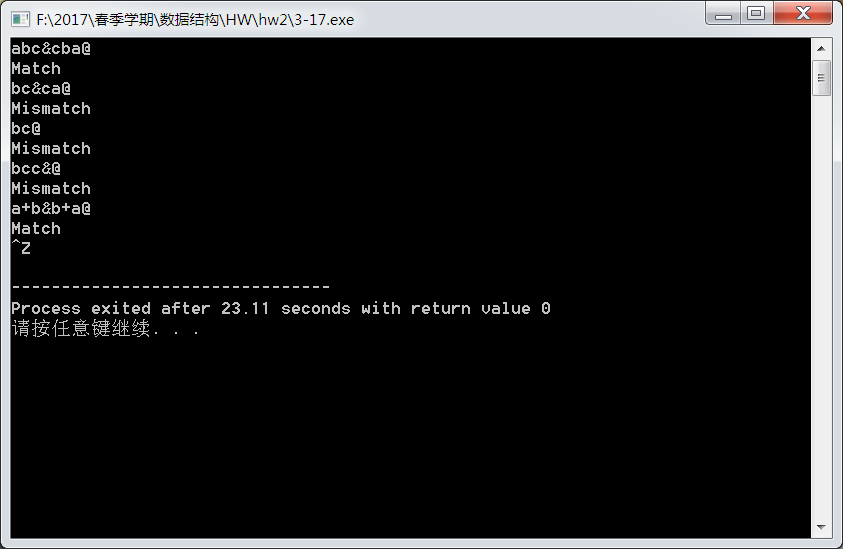
\includegraphics[width=0.75\textwidth]{hw2/screenshot/3-17}}
	\item[3.20](Flood-Fill算法,栈实现)
	\lstinputlisting[language=C]{hw2/3-20.c}
	
	读入一个$4\times 4$图像
	\[\begin{matrix}
	1 & 2 & 3 & 4\\
	2 & 2 & 2 & 3\\
	1 & 2 & 2 & 4\\
	3 & 2 & 2 & 2
	\end{matrix},\]
	以$(1,1)$为原点,将同一区域中点的颜色由$2$置换为$7$:
	
	\mbox{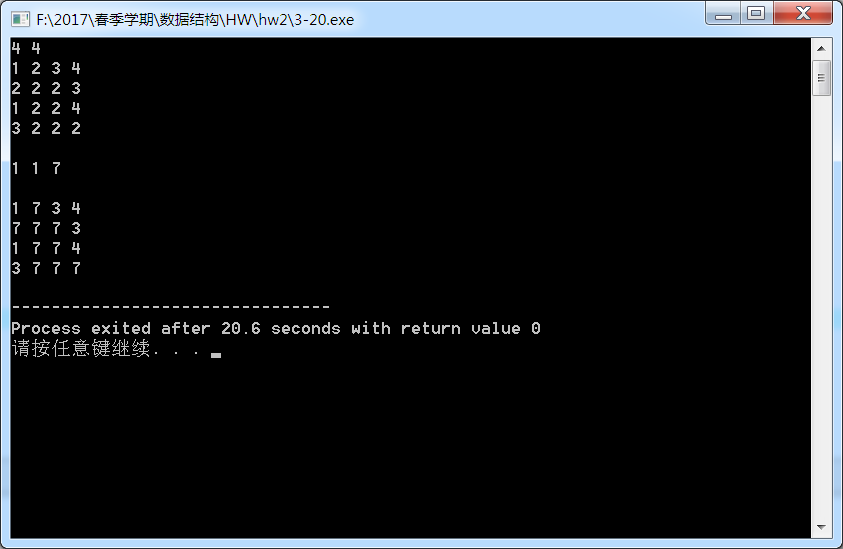
\includegraphics[width=0.75\textwidth]{hw2/screenshot/3-20}}
	\item[3.21]代码如下.
	\lstinputlisting[language=C]{hw2/3-21.c}
	
	将表达式\texttt{(a+b)*c-d}转为逆波兰表达式(以井号结尾):
	
	\mbox{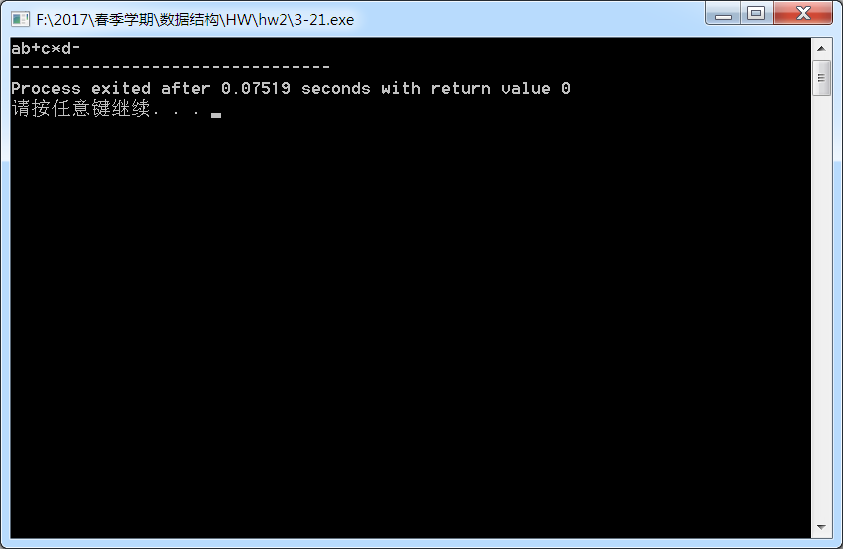
\includegraphics[width=0.75\textwidth]{hw2/screenshot/3-21}}
	\item[3.25]递归代码如下:
	\lstinputlisting[language=C]{hw2/3-25-recursive.c}
	试求$F(0)$至$F(9)$如下:
	
	\mbox{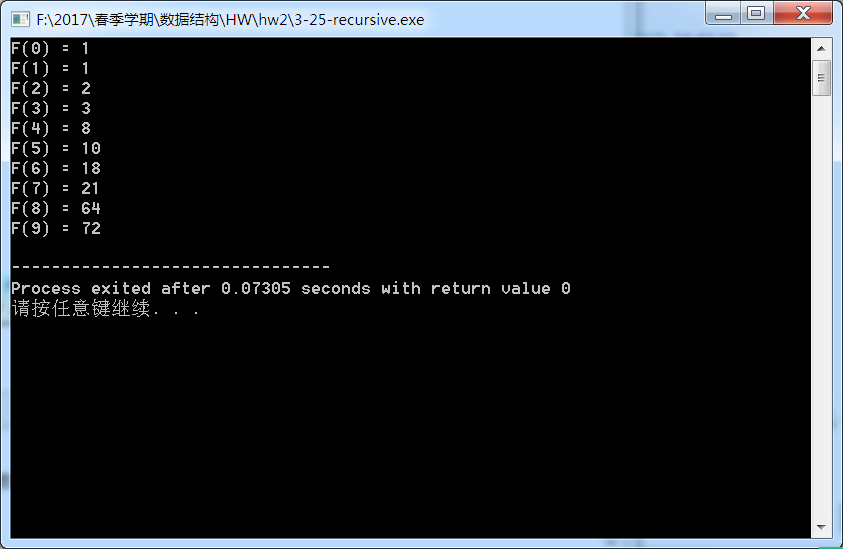
\includegraphics[width=0.75\textwidth]{hw2/screenshot/3-25-recursive}}
	
	改为非递归如下:
	\lstinputlisting[language=C]{hw2/3-25-nonrecursive.c}
	试求$F(0)$至$F(9)$如下,结果同上:
	
	\mbox{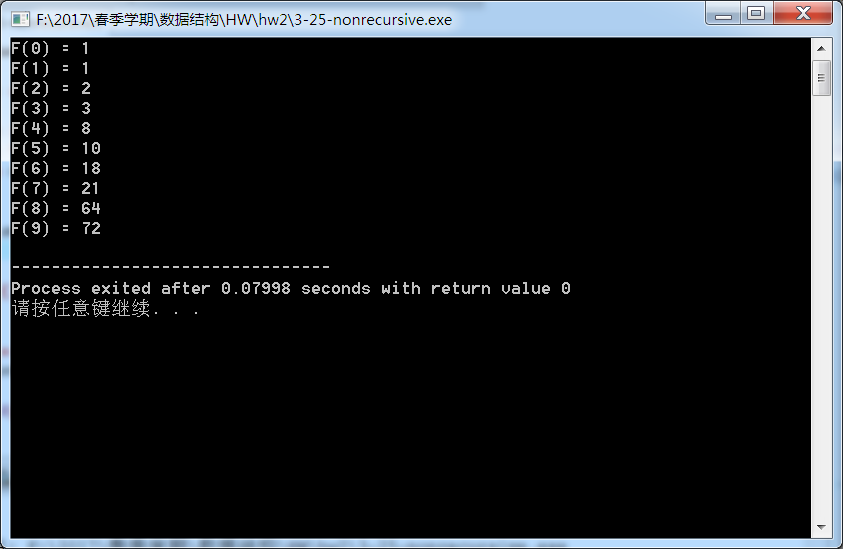
\includegraphics[width=0.75\textwidth]{hw2/screenshot/3-25-nonrecursive}}
	\item[3.31]代码如下.
	\lstinputlisting[language=C]{hw2/3-31.c}
	
	依次测试下列字符串:\fbox{\texttt{abba@}},\fbox{\texttt{abcba@}},\fbox{\texttt{abcde@}},\fbox{\texttt{ababab@}}:
	
	\mbox{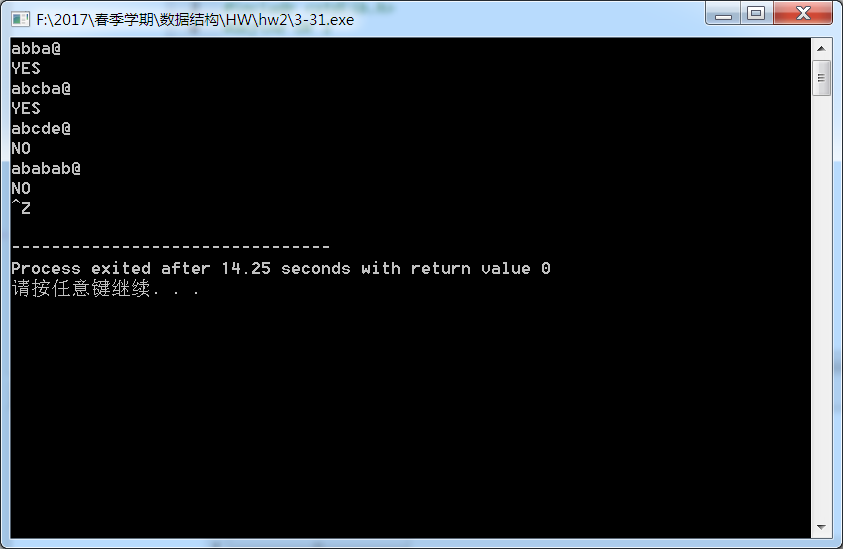
\includegraphics[width=0.75\textwidth]{hw2/screenshot/3-31}}
\end{enumerate}
\end{document}